\chapter{Phân tích và thiết kế hệ thống}

\section{Phân tích yêu cầu}
    \subsection{Yêu cầu người dùng}
    	\begin{itemize}
				\item Đối với người dùng
					\begin{itemize}
				        \item Đăng kí, đăng nhập đổi mât khẩu cho người dùng.
				        \item Chỉnh sửa thông tin cá nhân: Người dùng có thể dễ dàng thay đổi thông tin cá nhân của mình.
				        \item Tạo đơn hàng: Lúc tạo đơn hàng người dùng có thể tự đến gửi hàng trực tiếp tại kho hoặc người dùng chọn option có tài xế đên lấy, phí vận chuyển có thể là người gửi thanh toán hoặc ngườiTrong nhận thanh toán.
				        \item Chỉnh sửa đơn hàng: Trong thời gian đơn hàng chưa được xác nhận bởi tài xế thì người dùng có thể chỉnh sửa một số thông tin như địa chỉ giao nhận, khối lượng hàng hoá, loại hàng hóa,...
				        \item Hủy đơn hàng: Trong khoảng thời gian đơn hàng được xác nhận bởi tài xế thì đơn hàng có thể bị hủy. Chú ý rằng sau khi đơn hàng đã được xác nhận thì người dùng không thể hủy, nếu bắt buộc phải hủy thì người dùng vẫn phải chịu chi phí vận chuyển.
				        \item Xem danh sách các đơn hàng: Người dùng có thể dễ dàng xem thông tin đơn hàng. Danh sách đơn hàng có thể được lọc theo trạng thái, theo mã đơn hàng hoặc theo từng khoảng thời gian khác nhau nhanh chóng.
				        \item Xem nợ công và thanh toán: Người dùng có thể xem các đơn hàng đã hoàn tất và tiến hành thanh toán trung gian qua Ví điện tử hoăc thẻ ngân hàng.
				        \item Nhận thông báo: Sau khi đơn hàng được xác nhận bởi tài xế, thì ngươi dùng sẽ liên tục nhận được thông báo mỗi khi chuyển trạng thái của đơn hàng. Điều này giúp cho người dùng có thể theo dõi đơn hàng chặt chẽ và dễ dàng dự báo thời gian nhận hàng của mình.
				        \item Tìm kiếm đơn hàng: Đối với người nhận không phải là user của hệ thống thì vẫn có thể dễ dàng xem thông tin các đơn hàng thông qua số điện thoại của mình.
				        \item Yêu cầu hỗ trợ: Khi có các vấn đề thắc mắc thì người dùng có thể gửi yêu cầu để quản lý trực tiếp phản hồi. Danh sách các yêu cầu có thể được lọc theo mã yêu cầu, ngày, tháng, năm.
				        
				    \end{itemize}
				
			         
				\item Đối với tài xế
	                \begin{itemize}
	                    \item Đăng nhập đổi mât khẩu cho tài xế.
	                    \item Chỉnh sửa thông tin cá nhân: Tài xế có thể dễ dàng thay đổi thông tin cá nhân của mình.
	                    \item Nhận đơn hàng: Sau khi đơn hàng được tạo ra thì tài xế có thể nhận đơn và tiến hàng vận chuyển hàng hóa.
	                    \item Xem danh sách kiện hàng cần lấy: Hệ thống sẽ tự động gán đơn đối với tài xế liên tỉnh và tài xế đi giao cho nên tài xế cần theo dõi danh sách đơn hàng cần lấy để lấy đúng kiện hàng mà mình vận chuyển.
	                    \item Xem danh sách kiện hàng cần giao: Tài xế có thể xem thông tin chi tiết về các đơn hàng mà mình cần giao.
	                    \item Xác nhận đơn hàng với người dùng: Trong quá trình giao nhận hàng giữa tài xế và người dùng (người nhận, người gửi) thì tài xế đều phải xác nhận đơn hàng để 
	                    \item Báo cáo vấn đề: Trong quá trình vận chuyển có thể xảy ra các vấn đề ngoài ý muốn như: làm thất lạc hàng, gặp sự cố ngoài ý muốn không thể đảm bảo thời gian giao hàng,... thì tài xế có thể báo cáo lên để quản lý có thể giải quyết.
	                    \item Nhận thông báo: Mỗi khi đơn hàng được gán cho tài xế thì sẽ có mail thông báo cho tài xế. Việc nay giúp tài xế nắm thông tin đơn hàng, đảm bảo việc giao nhận diễn ra kịp thời.
	                \end{itemize}
	                
	                
				\item Đối với thủ kho
			    	\begin{itemize}
			    	    \item Đăng nhập đổi mât khẩu cho thủ kho.
			    	    \item Chinh sửa thông tin thủ kho.
	                    \item Nhập kho: Sau khi đơn hàng vận chuyển đến kho thì thủ kho có trách nhiệm xác nhận đơn hàng đúng về số lượng và đảm bảo chất lượng nguyên vẹn. Sau khi xác nhận thì tiến hành nhập kho để lưu trữ và phân phối tiếp tục cho tài xế.
	                    \item Xuất kho: Sau khi đơn hàng đã phân phối cho tài xế thì thủ kho có trách nhiệm kiểm tra hàng một lần nữa và bàn giao cho tài xế. 
	                    \item Xuất hóa đơn: Trong quá trình nhập kho và xuất kho thì thủ kho có thể xuất hóa đơn để xác nhận đã nhập hàng hoặc bàn giao hàng hóa cho tài xế.
	                    \item Xem danh sách đơn hàng: Thủ kho có thể xem danh sách đơn hàng đang ở trong kho mà mình quản lý. Danh sách đơn hàng được lọc theo mã hoặc có thể theo ngày, tháng, năm.
	                \end{itemize}
	                
	                
				\item Đối với quản lý
				    \begin{itemize}
	                    \item Đăng nhập đổi mât khẩu cho quản lý.
	                    \item Tạo tài khoản cho tài xế: Quản lý có thể tạo tài khoản và phân kho cho tài xế khi tài xế mới nhận việc.
	                    \item Xem biểu đồ thống kê: Quản lý có thể xem biểu đồ thống kê về tình hinh hoạt động của các kho, tình hình vận chuyển hàng hóa.
	                    \item Xử lý sự cố: Khi nhận được sự cố từ tài xế thì quản lý có thể xử lý sự cố và cập nhật trạng thái đơn hàng cho người dùng.
	                    \item Xử lý yêu cầu từ người dùng: Khi người dùng yêu cầu thì quản lý có thể phản hồi thắc mắc hoặc các phản ánh tử người dùng.
	                \end{itemize}
		\end{itemize}
    
    \subsection{Yêu cầu hệ thống}
    Hệ thống vận chuyển hàng hóa liên tỉnh cần đáp ứng một số yêu cầu về hệ thống như sau:
        \begin{itemize}
            \item Thời gian xử lý mỗi request từ người dùng không quá 1s
            \item Hệ thống gửi thông báo cho người dùng hoặc tài xế  không quá 5s
            \item Hệ thống có thể chịu tải 100req/s
            \item Thời gian tải hóa đơn nhập hàng/xuất hàng không quá 2s
            \item Hệ thống cần mã hóa thông tin giao tiếp giữa client và server
            \item Hệ thống phải được thiết kế để khi có nhu cầu mở rộng, thêm tính năng mới phải dễ dàng.
            \item Hệ thống cân xuất thống kê về số lượng đơn hàng được vận chuyển thành công, thất bại, doanh thu vào ngày cuối cùng trong tháng.
        \end{itemize}
    
    \newpage

\section{Thiết kế hệ thống}

\subsection{Kiến trúc hệ thống}
	
		\begin{figure}[!ht]
			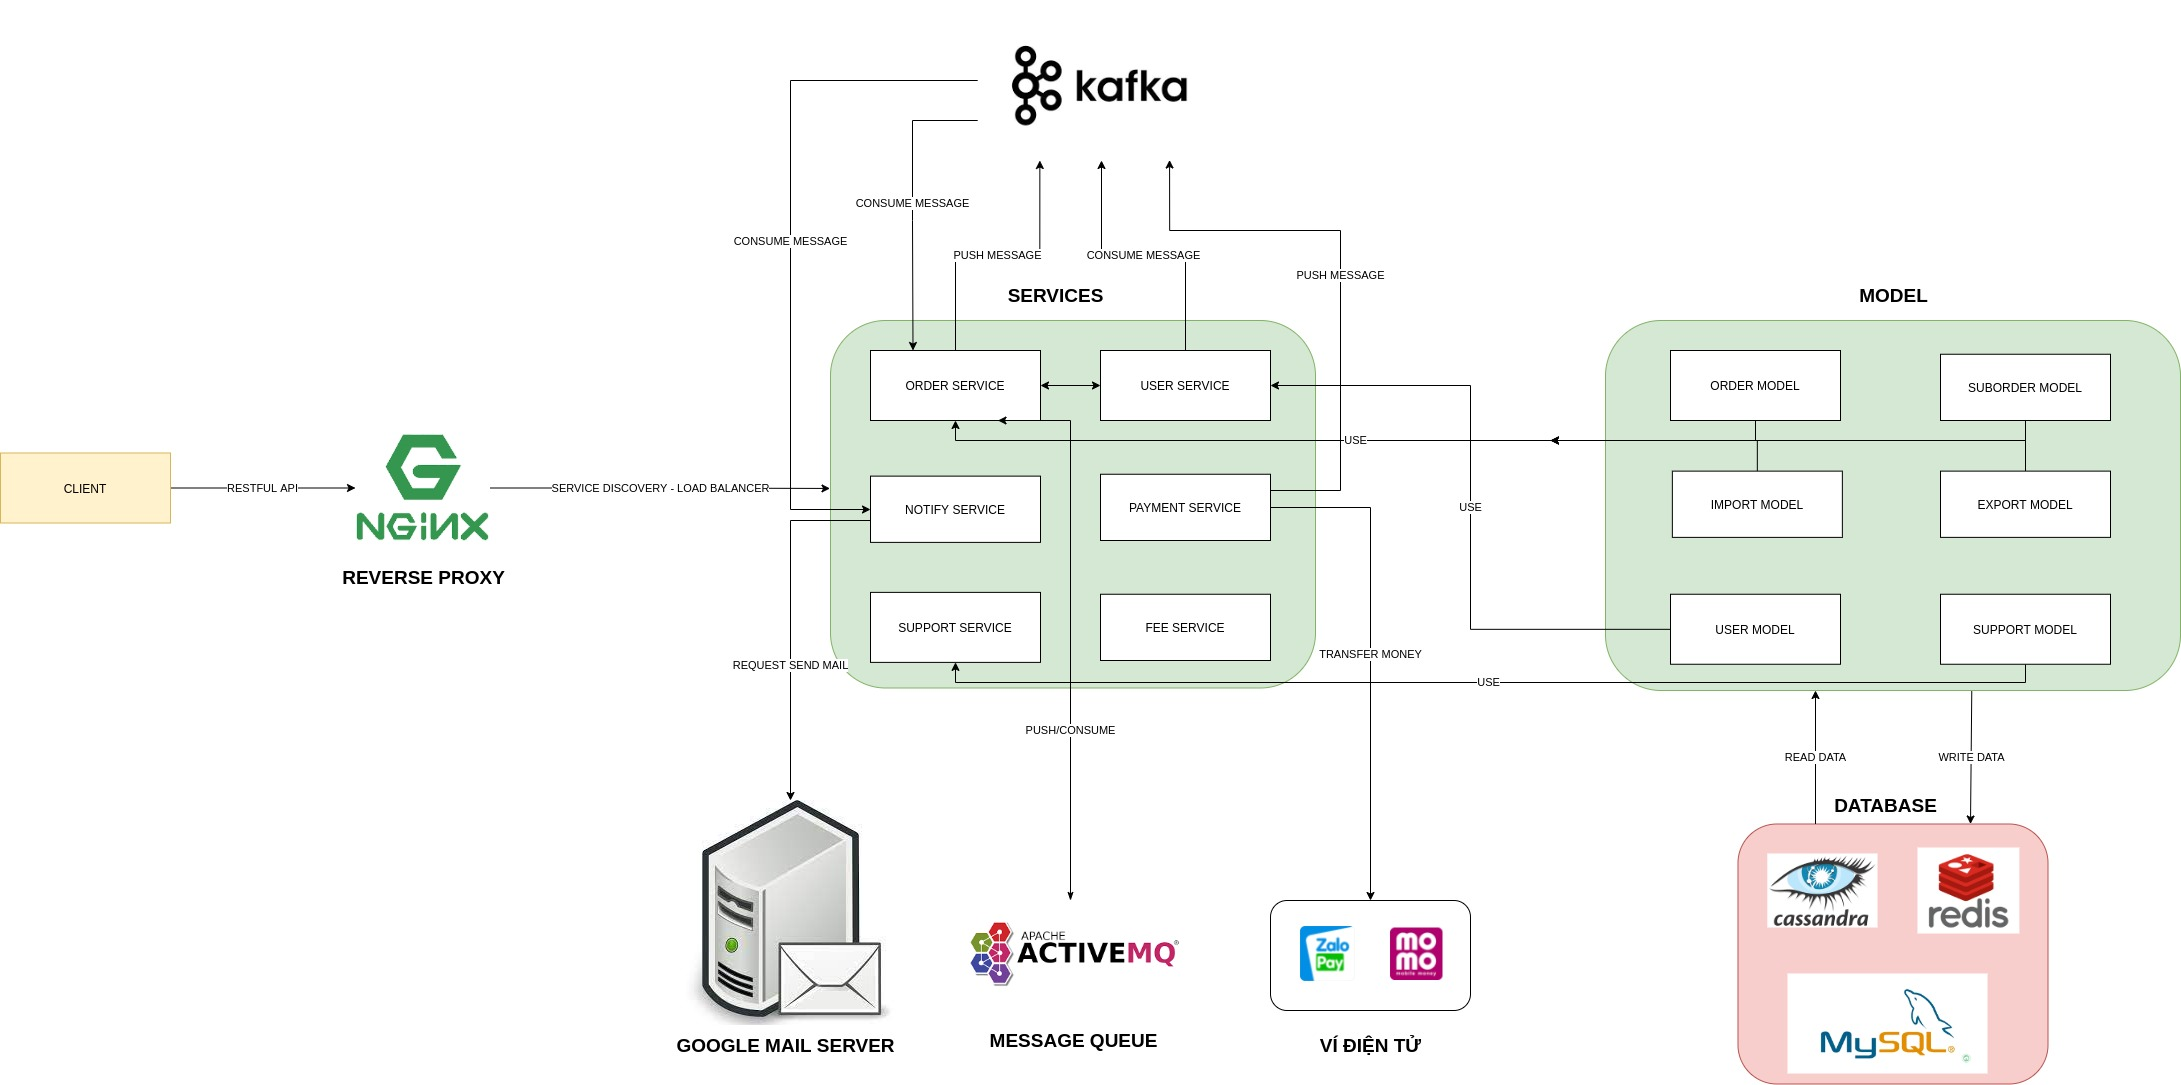
\includegraphics[width=1\textwidth]{Images/SystemArchitecture.jpg}
			\centering
			\linebreak
			\caption{Kiến trúc hệ thống}
		\end{figure}
	

		
		\begin{itemize}
			\item \textbf{User Service}
			\begin{itemize}
				\item Service chịu trách nhiệm quản lý user trong hệ thống. Ở đây sẽ lưu trữ Database của user
				\item Mỗi khi user login vào hệ thống thì sẽ vào Service này để authen: Ban đầu user được yêu cầu sẽ nhập username và password, Sau khi authen là đúng user đó thì hệ thống sẽ sinh ra JWT (Json Web Token) để gửi trả về cho user. Sau này cứ mỗi request lên hệ thống thì user sẽ gửi kèm theo JWT để hệ thống có thể authen và author.
				\item User có thể get thông tin để có thể xem và chỉnh sửa
			\end{itemize}
			\item \textbf{Order Service}
			\begin{itemize}
				\item Service chịu trách nhiệm tạo, xử lý, lưu trữ các thông tin về đơn hàng cho User.
				\item Ngoài ra service còn chịu trách nhiệm phân phối các đơn hàng đến tài xế
				\item Đây là service chịu tải khá lớn trong hệ thống vì nhóm sử dụng kết hợp các giải pháp sau nhằm tăng hiệu suất cho service: 
					\begin{itemize}
						\item Sử dụng Message Queue để hiện thực cơ chế bất đồng bộ cho các tác vụ: Tạo đơn hàng, ghi dữ liệu vào Database.
						\item Sử dụng Kafka để gửi message cho service khác
						\item Trong quá trinh xử lý thì dữ liệu của đơn hàng được lưu trên Cache. Đến khi nào có \textbf{trạng thái cuối} thì đơn hàng mới được lưu vào Database. Bởi vì đơn hàng đươc lấy và thay đổi trạng thái rất nhiều lần trong quá trình xử lý, nếu ghi vào Database (thực hiện nhiều I/O operations) sau mỗi lần xử lý như vậy thì sẽ làm giảm performance rất nhiều. Việc xử lý dữ liệu trên Cache cũng có thể gặp rủi ro như Cache Server sập thì dữ liệu có thể mất hết, nhưng rất may Redis có hỗ trợ cơ chế Persistence (định kỳ sao lưu dữ liệu) nên rủi ro này có thể chấp nhận được.
					\end{itemize}
				\item Mỗi khi đơn hàng thay đổi trạng thái hoăc tài xế đươc phân phối đơn thì service sẽ produce message vào \textbf{Kafka Broker} để \textbf{Notify Service} consume và tiếp tục xử lý
			\end{itemize}
			\item \textbf{Notify Service}
			\begin{itemize}
				\item Service chịu trách nhiệm quản lý các thông báo cho hệ thống.
				\item Service sẽ consume message tử \textbf{Order Service} và gửi yêu cầu về mail cho \textbf{Google Mail Server}.
				\item Hệ thống sẽ gửi thông báo mỗi khi: 
					\begin{itemize}
						\item Gửi thông báo cho khách hàng mỗi khi trạng thái đơn hàng thay đổi. 
						\item Gửi thông báo cho tài xế mỗi khi được phân phối đơn.
						\item Gửi mã xác thực OTP
					\end{itemize}
			\end{itemize}
			\item \textbf{Fee Service}
			\begin{itemize}
				\item Service chịu trách nhiệm hiện thực giải thuât, công thức để tính toán các khoản phí phát sinh cho khách hàng.
				\item Database lưu thông tin về phí của mỗi đơn hàng để các user có thể đối soát.
			\end{itemize}
			\item \textbf{Payment Service}
			\begin{itemize}
				\item Service này sẽ liên kết với 1 bên thứ 3 như: ngân hàng, ví điện từ, .... để thực hiện chức năng thanh toán cho các user.
			\end{itemize}
			\item \textbf{Reverse Proxy}
			\begin{itemize}
				\item Hệ thống sử dụng NGINX như là một \textbf{Reverse Proxy} nhằm thực hiện một số chức năng như: 
				\begin{itemize}
					\item \textbf{Bảo mât}: Kiểm soát các yêu cầu của Client gửi tới, nếu hợp lệ sẽ luân chuyển đến các service bên trong để xử lý. Che giấu địa chỉ IP của các service bên trong nhằm giúp các service trách khỏi các cuôc tấn công mạng. Ngoài ra còn có thể dễ dàng thiết lập SSL nhằm mã hóa dữ liệu trong quá trình giao tiếp giữa Client và các service bên trong.
					\item \textbf{Cân bằng tải}: Mỗi service có thể được deploy với nhiều instance để có thể chịu tải cao hơn. Reverse proxy sẽ thực hiện một số giải thuật như: Round Robin, Least Connection, ... để đẩy các request vào cho các service xử lý.
				\end{itemize}
			\end{itemize}
			
				\item Database
				\begin{itemize}
					\item \textbf{MySQL}: Hệ thống sử dụng MySql để lưu các thông tin ít được truy xuất như log, cấu hình service,...
					\item \textbf{Cassandra}: Với khả năng đọc/ghi có tốc độ nhanh cùng với đó là khả năng chịu lỗi cao hệ thống sử dụng Cassandra để lưu các thông tin về Order, Hóa đơn nhập/xuất kho,...
					\item \textbf{Redis}: Với Redis thì dữ liệu được lưu trữ trong memory vì thế giúp cho service truy xuất thông tin rất nhanh chóng. Hệ thống sẽ lưu các thông tin thường xuyên được truy xuất bởi user như thông tin về yêu cầu, đơn hàng,... Ngoài ra còn tận dụng cấu trúc dữ liệu đa dạng trong Redis để giải quyết một số bài toán phức tạp. 
				\end{itemize}
		
		\end{itemize}

\newpage
\subsection{Thiết kế Use Case}

\begin{figure}[!ht]
	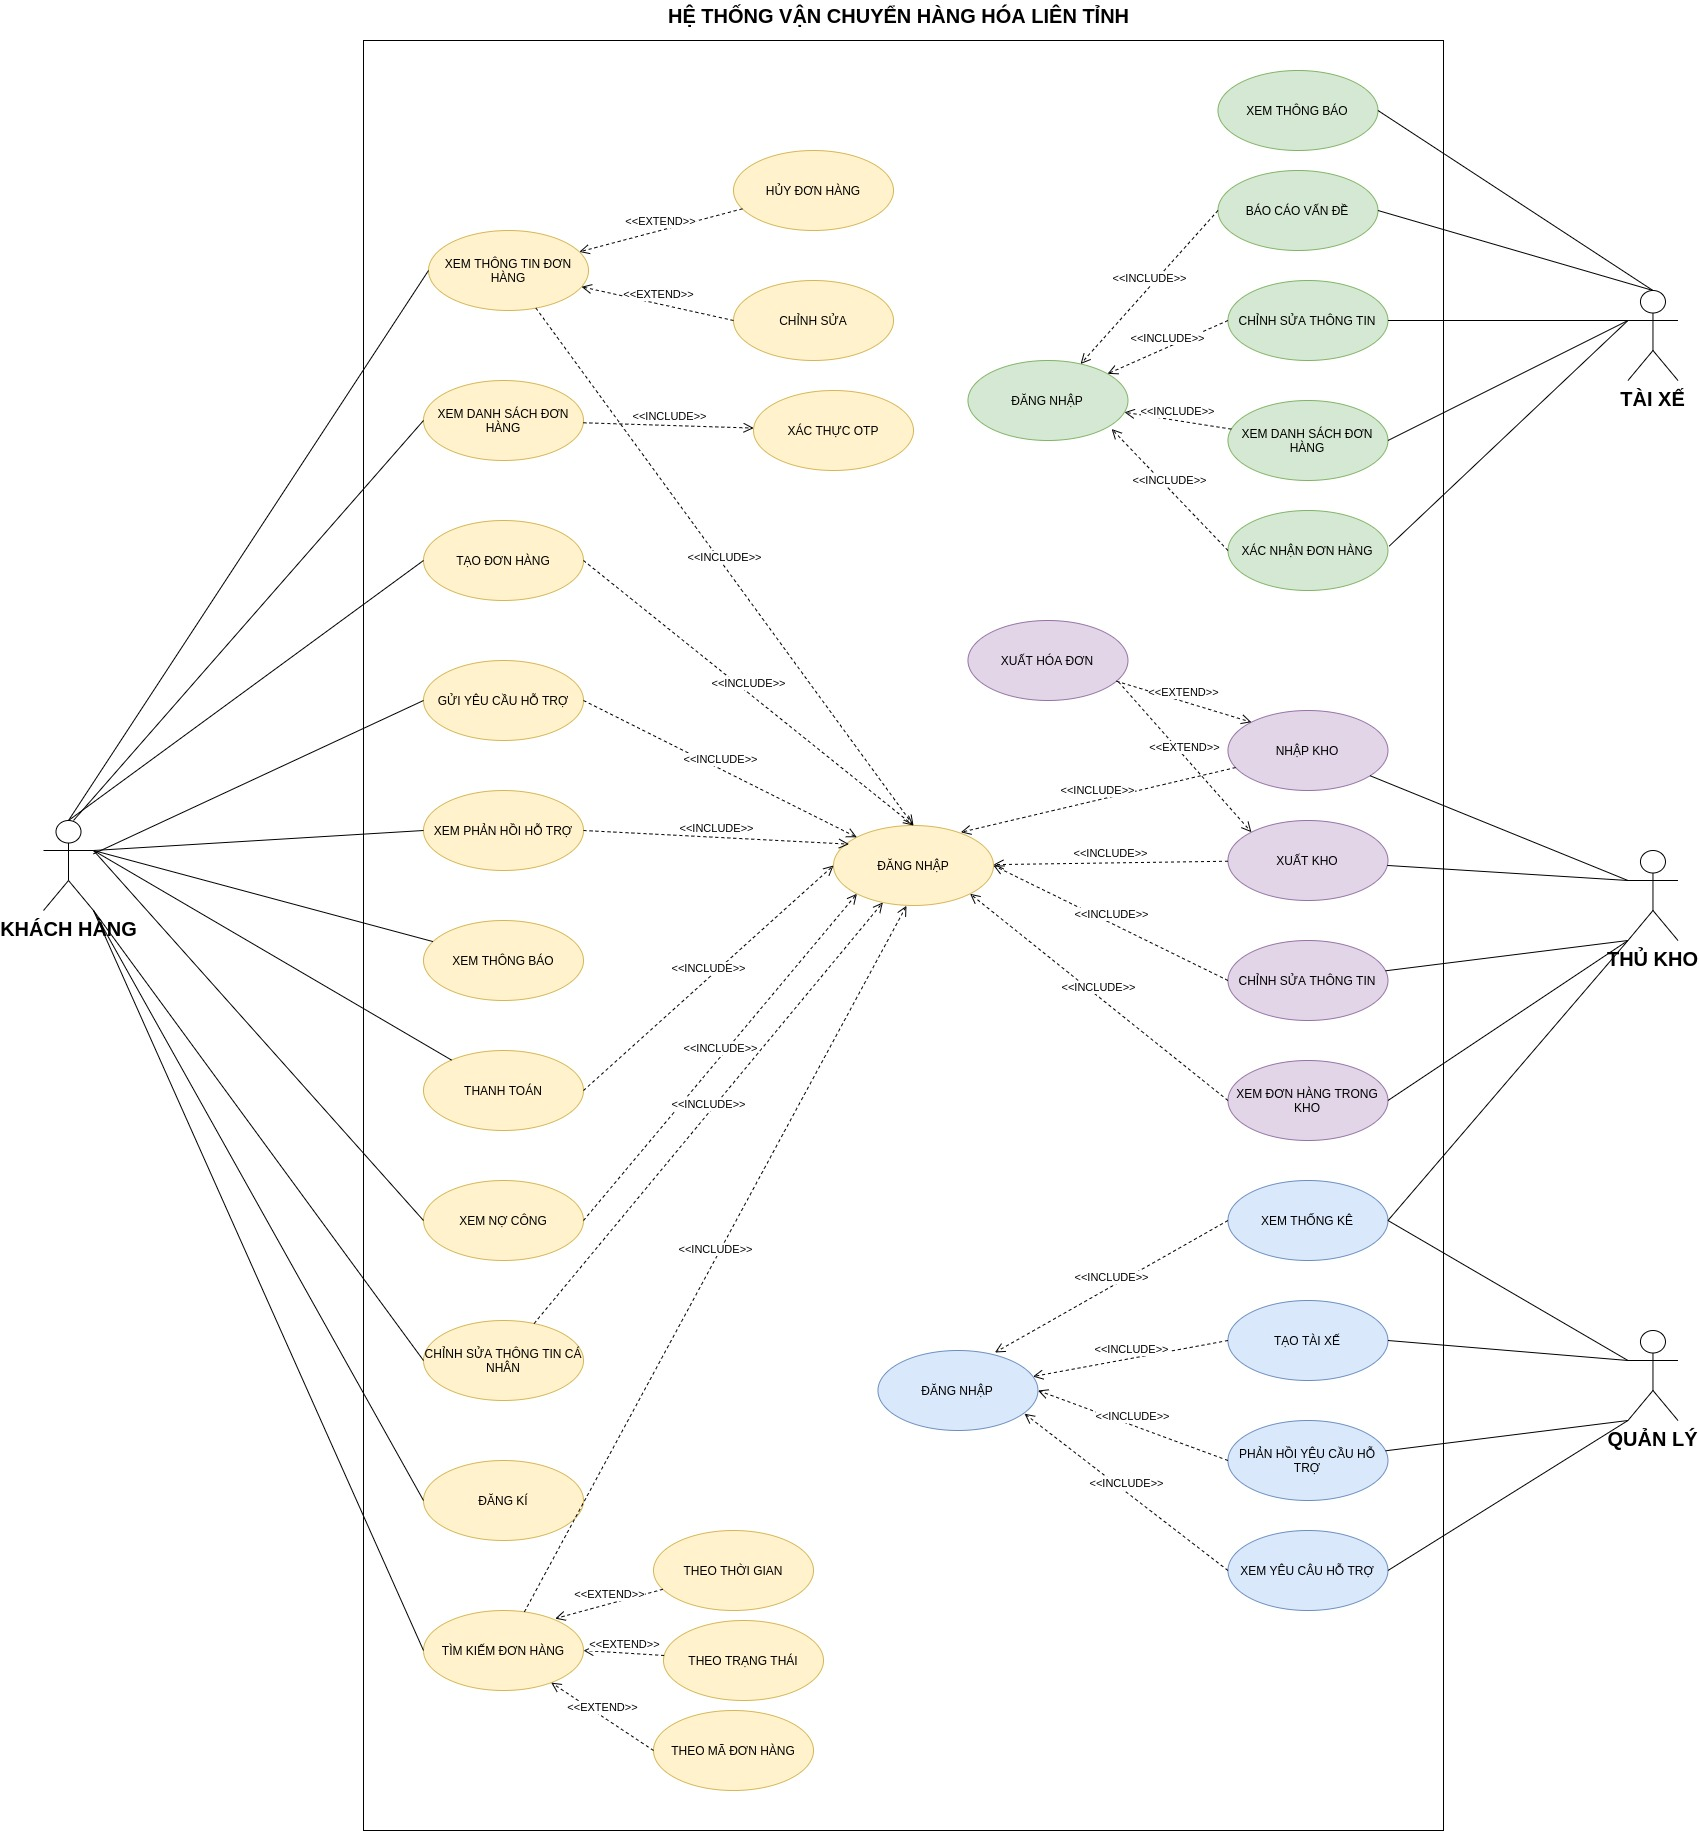
\includegraphics[width=1\textwidth]{/UseCase.jpg}
	\centering
	\linebreak
	\caption{Sơ đồ Use case}
\end{figure}

\begin{itemize}
	\item 
% 	\subsection{Trạng thái đơn hàng}
	\begin{itemize}
		\item Đơn nháp: Trạng thái đầu, khi người dùng tạo yêu cầu đơn hàng
		\item Chờ bàn giao: Khi người dùng ấn nút gửi yêu cầu. Cho phép tối đa 30s để người dùng có thể chỉnh sửa hoặc hủy đơn (Có thể nhấn nút submit để chốt sớm hơn). Sau thời gian đó đơn hàng sẽ chuyển status sang trạng thái kế tiếp
		\item Trong hàng chờ phân phối: Đưa vào hàng chờ của hệ thống phân phối (Chi tiết ghi trong actor "Hệ thống phân phối")
		\item Đang lấy hàng: Các kiện hàng của đơn hàng đã và đang được đến lấy về kho (Có thông tin thêm là <x / tổng số kiện hàng> đã được lấy).
		\item Đã vào kho tập trung <Địa điểm 1>: Các kiện hàng của đơn hàng đã được lấy hết và được đưa vào kho <Địa điểm 1> 
		\item Đang giao liên tỉnh: Đơn hàng đã xuất kho 1 và đang được giao liên tỉnh từ kho 1 đến kho 2
		\item Đã vào kho tập trung <Địa điểm 2>: Các kiện hàng của đơn hàng đã được lấy hết và được đưa vào kho <Địa điểm 2>
		\item Đang giao hàng: Các kiện hàng của đơn hàng đã và đang được giao đến người nhận cuối
		\item Hoàn tất: Khi tất cả các kiện hàng của đơn hàng đã đến địa điểm cuối
		\item Đơn hủy: Trạng thái khi khách hàng hủy đơn ở trạng thái chờ bàn giao (Khách hàng chỉ được hủy ở trạng thái chờ bàn giao).
	\end{itemize}
% 	\subsection{Người gửi}
	\begin{itemize}
		\item \textbf{Tạo đơn hàng:} Người gửi cần điền những thông tin sau: 
		\begin{itemize}
			\item Bên gửi:
			\begin{itemize}
				\item Tên người gửi
				\item Số điện thoại
				\item Địa chỉ, chia làm 3 phần gồm Số địa chỉ + tên đường, Quận - Huyện, Phường - Xã. Quận - Huyện và Phường - Xã được nhập bằng cách chọn trong một dropdown có sẵn.
			\end{itemize}
			\item Bên nhận:
			\begin{itemize}
				\item Tên người nhận
				\item Số điện thoại
				\item Địa chỉ, tương tự như bên gửi.
			\end{itemize}
			\item Thông tin về (các) món hàng muốn gửi:
			\begin{itemize}
				\item Tên sản phẩm + số lượng (Mặc định là 1). Có thể thêm nhiều sản phẩm và có thể chỉnh sửa số lượng của từng sản phẩm đã thêm.
				\item Khối lượng (Để tính phí vận chuyển). Nhân viên đến lấy hàng sẽ tiến hành xác nhận bằng cách đo lại và sẽ yêu cầu khách hàng cập nhật lại khối lượng nếu như khối lượng đã nhập trước đó là không chính xác.
				
			\end{itemize}
			\item Lựa chọn cho bên nhận:
			\begin{itemize}
				\item Không cho xem hàng.
				\item Cho xem hàng nhưng không cho thử.
				\item Cho thử hàng.
			\end{itemize}
			\item Lựa chọn tính phí cho bên gửi hoặc bên nhận 
			\item Lựa chon gửi hàng / nhận hàng tại kho sẽ không tính phí nội tỉnh(phí liên tỉnh luôn có ). Ngược lại sẽ tính phí nội tỉnh (gửi và nhận giống nhau). 
			\item Hệ thống sẽ tự tính cước vận chuyển dựa trên khoảng cách bên gửi/nhận và khối lượng món hàng.
			\item Các thông tin ghi chú khác (Người gửi tự điền vào ô textbox).
			\item Mockup / Wireframe (Dự kiến tham khảo thiết kế UI của GHN):
		\end{itemize} 
		
		\begin{figure}[!ht]
			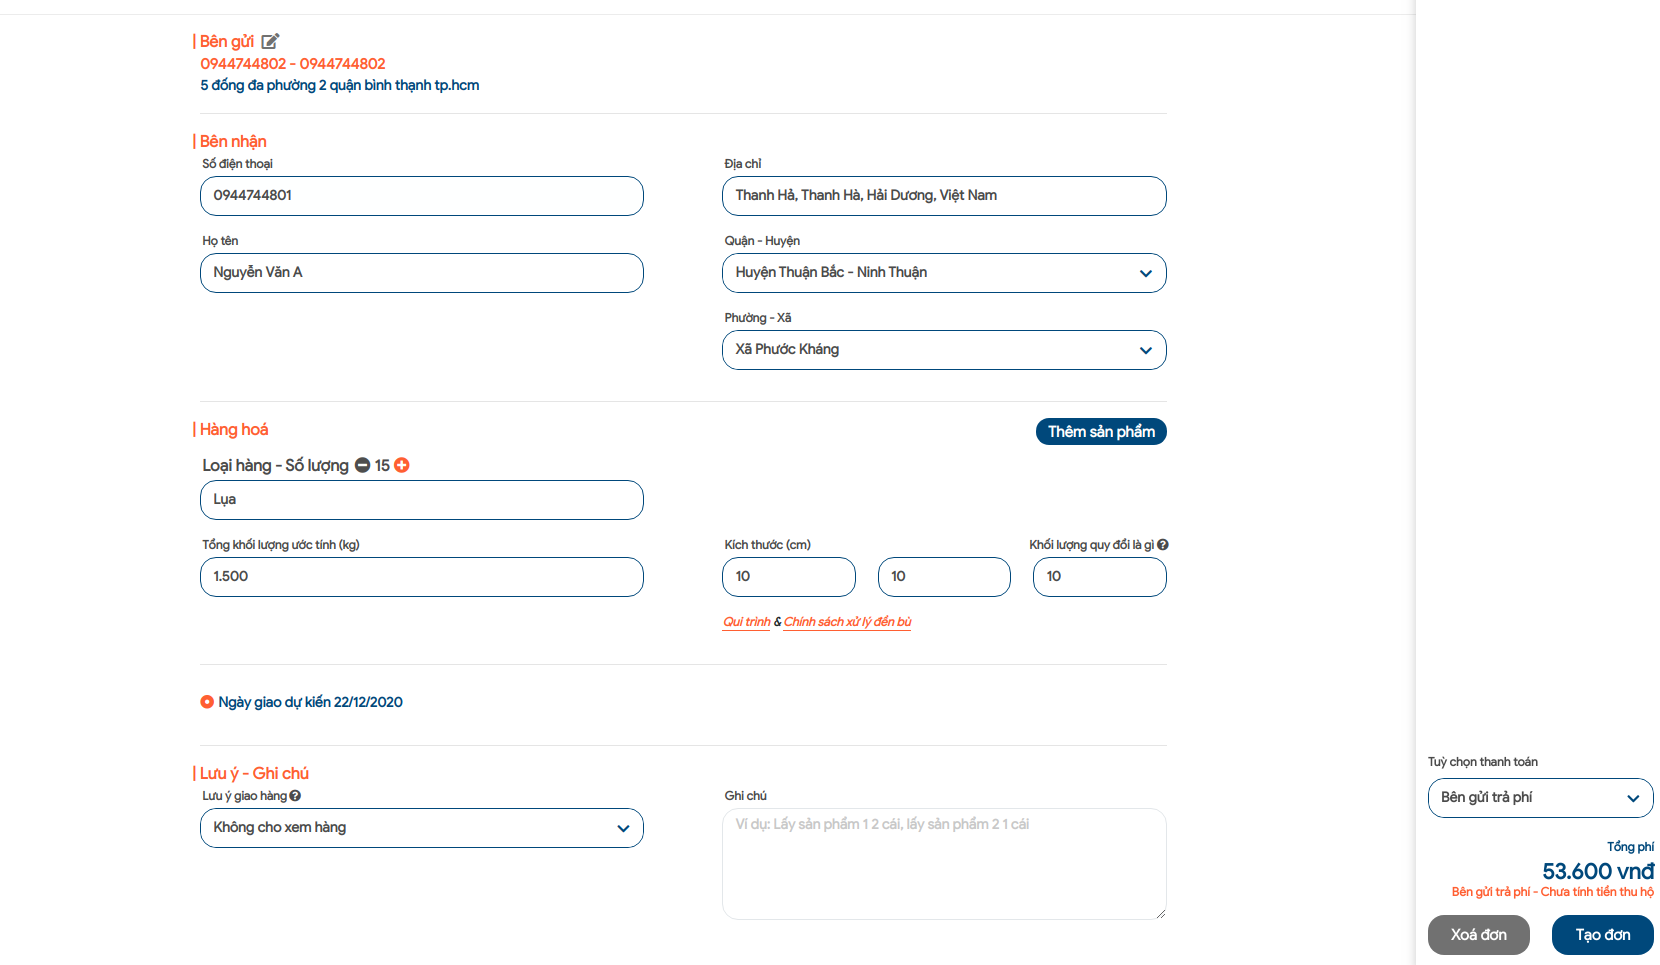
\includegraphics[width=1\textwidth]{/create-order.png}
			\centering
			\linebreak
			\caption{Giao diện tạo đơn hàng (dự kiến)}
		\end{figure}
		
		\item \textbf{Chỉnh sửa thông tin đơn hàng:} Nếu vẫn đang trong quá trình bàn giao và xác nhận(trong trạng thái \textbf{Chờ bàn giao}), người gửi có thể chỉnh sửa thông tin đơn hàng (Thông tin như trong mục tạo đơn, sẽ có giới hạn thông tin được chỉnh sửa).
		
		\item \textbf{Hủy đơn hàng:} Nếu vẫn đang trong quá trình bàn giao và xác nhận(trong trạng thái \textbf{Chờ bàn giao}), người gửi có thể hủy đơn hàng. Đơn hàng bị hủy sẽ được chuyển vào mục thùng rác và cho phép người dùng tái sử dụng thông tin của đơn hàng bị hủy ấy (Tạo lại đơn hàng mới dựa trên thông tin đơn hàng bị xóa ấy).
		
		\item \textbf{Xem danh sách các đơn hàng}: Các đơn hàng sẽ được chia theo trạng thái đã định nghĩa ở trên và người gửi có thể xem list các đơn hàng lọc theo trạng thái đó. Mockup / Wireframe (Dự kiến tham khảo thiết kế UI của GHN):
		
		\begin{figure}[!ht]
			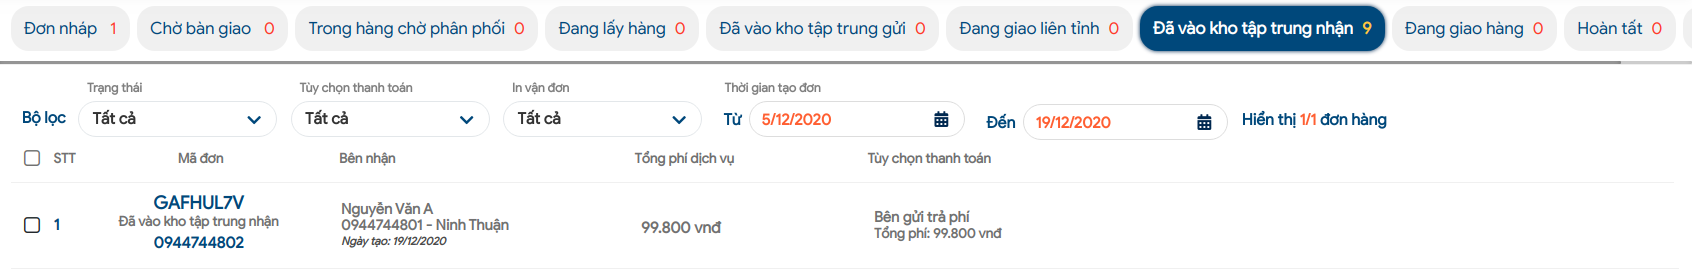
\includegraphics[width=1\textwidth]{/order-status.png}
			\centering
			\linebreak
			\caption{Giao diện xem danh sách các đơn hàng (dự kiến)}
		\end{figure}
		
		\item \textbf{Xem nợ công và thanh toán}: Do phí có thể được tính cho người gửi hoặc người nhận (theo nhu cầu của người gửi), người gửi và người nhận đều có thể xem nợ công và thực hiện thanh toán. Thanh toán dự định sẽ được thực hiện qua ZaloPay
	\end{itemize}
	
% 	\subsection{Người nhận}
	\begin{itemize}
		\item \textbf{Xem nợ công và thanh toán}: Tương tự UC của người gửi
		
		\item \textbf{Tra cứu thông tin đơn hàng:} Mỗi đơn hàng được tạo sẽ có một mã riêng biệt dùng cho người gửi/nhận tra cứu thông tin và tình trạng hiện tại của đơn hàng. Mockup / Wireframe (Dự kiến tham khảo thiết kế UI của GHN): 
		
		\begin{figure}[!ht]
			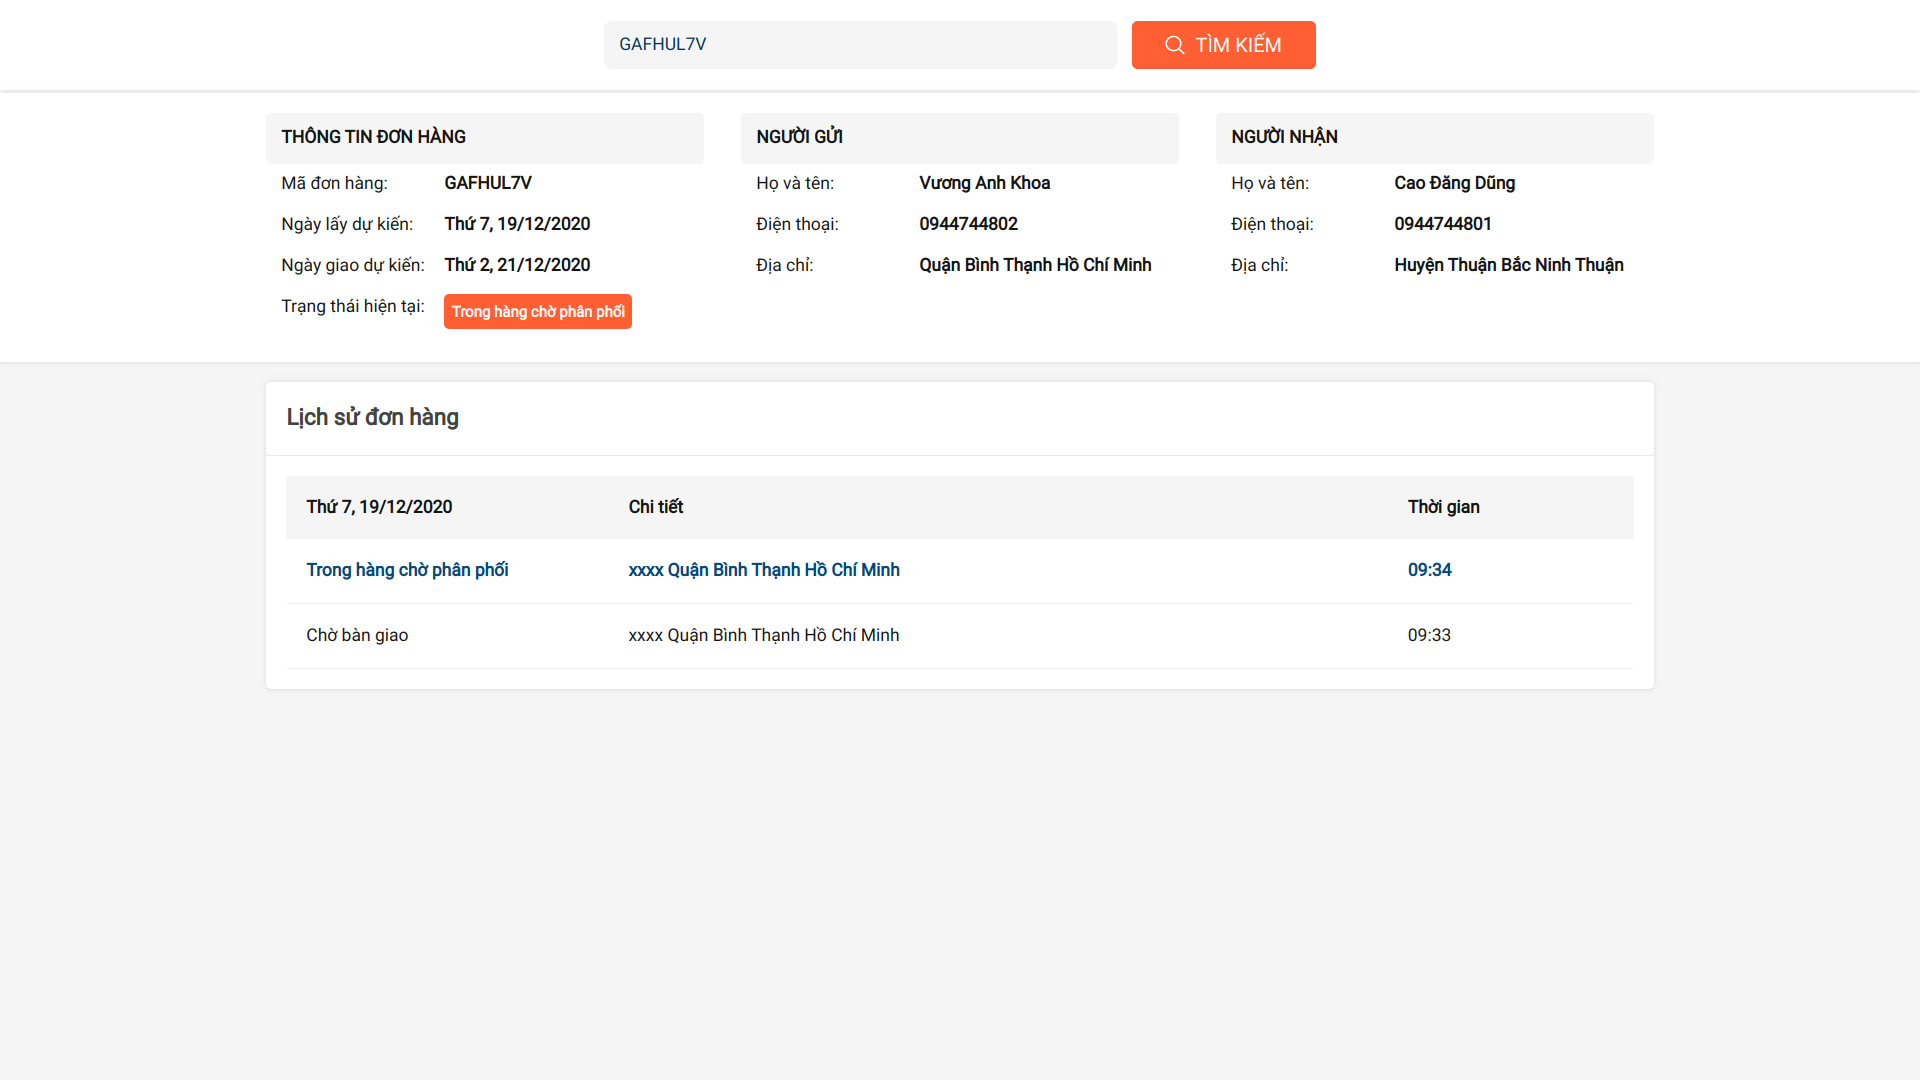
\includegraphics[width=0.95\textwidth]{/tracking.png}
			\centering
			\linebreak
			\caption{Giao diện theo dõi tình trạng đơn hàng (dự kiến)}
		\end{figure}
		
		\item \textbf{Xác nhận đơn hàng đã nhận}: Người nhận sẽ check vào những kiện hàng sẽ được nhận (trong đơn hàng của người nhận) có trong xe hoặc trong kho (nếu lựa là người nhận tự đến lấy). Nếu tất cả kiện hàng ở trong đơn hàng đã được check thì trạng thái đơn hàng cập nhật từ (Đang giao hàng -> Hoàn tất). Trong trường hợp nếu người nhận tự đến lấy thì sẽ có thêm khoản phí lưu kho (Được tính theo khoảng thời gian từ lúc đơn hàng nhập kho đến khi người nhận đến lấy).
	\end{itemize}
	
% 	\subsection{Tài xế nội tỉnh đi lấy}
	\begin{itemize}
		\item \textbf{Xem danh sách kiện hàng cần lấy:} Tài xế nội tỉnh sẽ được assign những kiện hàng cần đi lấy để thu gom về kho. Tài xế nội tỉnh có thể xem những thông tin cần thiết để tiến hành xử lí vận chuyển list danh sách các kiện hàng đó.
		
		\begin{figure}[!ht]
			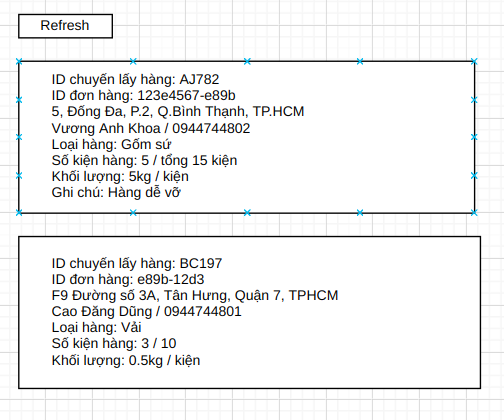
\includegraphics[width=0.7\textwidth]{/ntlay.png}
			\centering
			\linebreak
			\caption{Wireframe list các kiện hàng cần lấy của tài xế (dự kiến)}
		\end{figure}
		
		\item \textbf{Cập nhật nếu có thông tin sai sót}: Tài xế đến lấy hàng sẽ tiến hành đo lại và cập nhật thông tin kiện hàng nếu thông tin kiện hàng có sai sót (Như khối lượng, kích thước vv...). Sau đó, khách hàng sẽ tiến hành xác nhận lại thông tin tài xế cập nhật là chính xác để tiến hành giao nhận.
		
		\newpage
		
		\begin{figure}[!ht]
			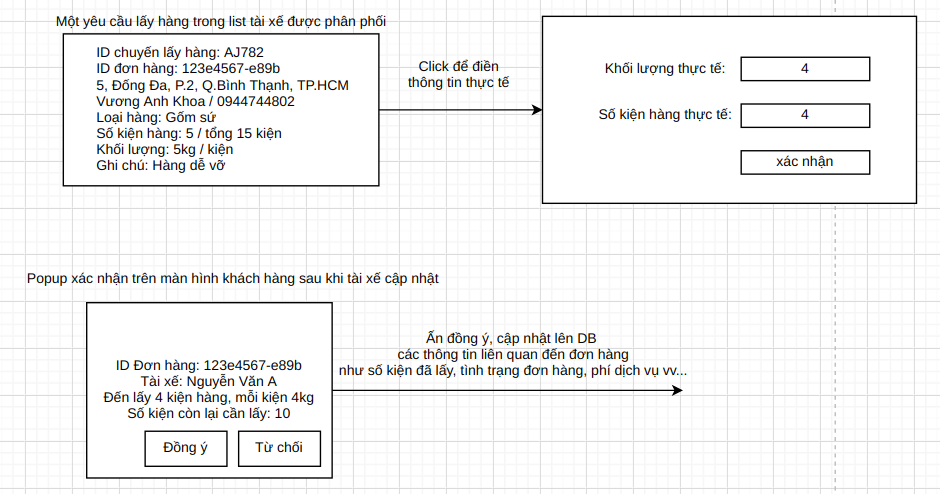
\includegraphics[width=1\textwidth]{/reconfirm.png}
			\centering
			\linebreak
			\caption{Wireframe miêu tả qui trình xác nhận thông tin sai sót}
		\end{figure}
	\end{itemize}
	
% 	\subsection{Tài xế nội tỉnh đi giao}
	\textbf{Xem danh sách kiện hàng cần giao}:  Tài xế nội tỉnh sẽ được assign những kiện hàng cần được giao cho người nhận. Tài xế nội tỉnh có thể xem những thông tin cần thiết để tiến hành xử lí vận chuyển list danh sách các kiện hàng đó.
	
% 	\subsection{Tài xế liên tỉnh} 
	\textbf{Xem danh sách kiện hàng cần lấy}: Tài xế liên tỉnh sẽ được assign những đơn hàng cần đi lấy để vận chuyển đến kho liên tỉnh. Tài xế liên tỉnh có thể xem những thông tin cần thiết để tiến hành xử lí vận chuyển list danh sách các đơn hàng đó.
% 	\subsection{Hê thống phân phối}
	\begin{itemize}
		\item \textbf{Phân phối đơn hàng cho tài xế nội tỉnh}: Các đơn hàng sẽ được đưa vào 2 loại hàng chờ (nội tỉnh): Hàng chờ hôm nay và hàng chờ các đơn hàng cho ngày hôm sau. Hệ thống qui định những kiện hàng được tạo trước <6h> tối sẽ được đưa vào hàng chờ hôm nay, còn những kiện hàng được tạo sau <6h> tối sẽ được đưa vào hàng chờ ngày hôm sau. Hệ thống sẽ chỉ phân phối các kiện hàng trong hàng chờ ngày hôm nay cho các tài xế nội tỉnh. Nếu hàng chờ ngày hôm nay chưa xử lí hết các kiện hàng thì sẽ được đẩy qua ngày hôm sau.Đơn vị ở đây là kiện hàng do xe nội tỉnh thường có kích thước nhỏ, không thể lấy hết cả 1 đơn hàng mà chỉ có thể lấy một số kiện hàng từ đơn ấy. Hệ thống sẽ cập nhật trạng thái từ <Trong hàng chờ phân phôi>  -->  <Đang lấy hàng>
		\item \textbf{Phân phối đơn hàng cho tài xế liên tỉnh}: Đơn hàng đã được tập kết đầy đủ (Tức toàn bộ kiện hàng của đơn hàng đã đến kho) sẽ được đưa vào hàng chờ liên tỉnh. Hệ thống qui định những đơn hàng đã được tập kết trước <12h> đêm sẽ được đưa vào hàng chờ hôm nay, còn những đơn hàng được tập kết sau <12h> đêm sẽ được đưa vào hàng chờ ngày hôm sau. Hệ thống sẽ chỉ phân phối các đơn hàng trong hàng chờ ngày hôm nay cho các tài xế liên tỉnh. Nếu hàng chờ ngày hôm nay chưa xử lí hết các đơn hàng thì sẽ được đẩy qua ngày hôm sau. Đơn vị ở đây là đơn hàng do xe liên tỉnh thường có kích thước lớn nên có thể chở cả 1 hoặc nhiều đơn hàng.
	\end{itemize}
	
% 	\subsection{Quản lí}
	
	\textbf{Xem thống kê}: Người quản lý có thể  xem thống kê về số lương đơn hàng trong tuần, tháng, năm thông qua biểu đồ; xem thống kê hiệu suất làm việc của tài xế ; số đơn hàng giao thành công và đơn hàng bị hủy trong tuần, tháng, năm.
	
	
% 	\subsection{Thủ kho}
	\begin{itemize}
		\item \textbf{Xem danh sách hàng trong kho}: Thủ kho sẽ xem list các đơn hàng có trong kho (Lọc theo tiêu chí tất cả, đơn hàng mà các kiện đã vào đủ, đơn hàng mà các kiện chưa vào đủ). Thông tin từng đơn hàng là loại hàng, <số kiện hàng đã vào kho / tổng số kiện>. 
		
		\begin{figure}[!ht]
			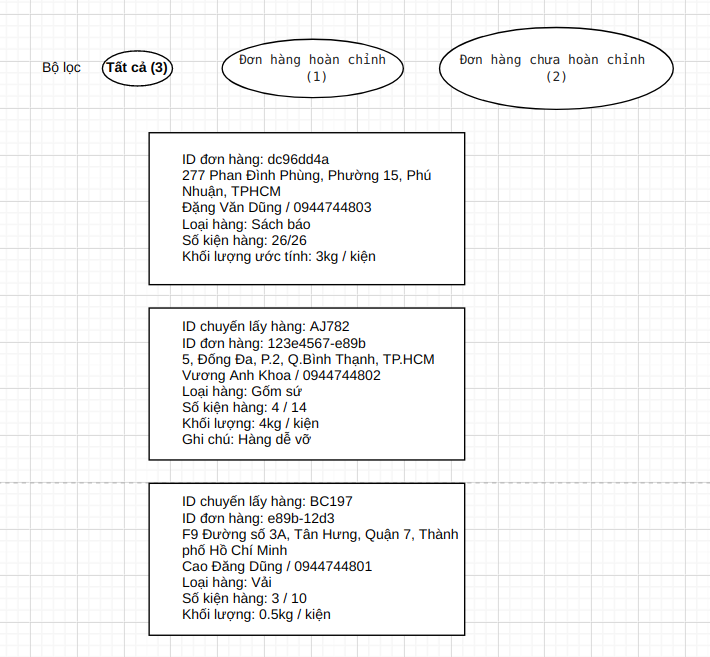
\includegraphics[width=0.75\textwidth]{/hangtrongkho.png}
			\centering
			\linebreak
			\caption{Wireframe xem danh sách hàng trong kho của thủ kho}
		\end{figure}
		
		\item \textbf{Xác nhận kiện hàng vào kho}:
		Khi tài xế nội tỉnh đến kho, thủ kho sẽ search ID của tài xế để xem list kiện hàng được phân công của tài xế Thủ kho sẽ kiểm tra xe của tài xế và check vào những kiện hàng thật sự có trong xe để hoàn tất quá trình nhập kho của kiện hàng. (Tức hệ thống sẽ cập nhật số kiện hàng đã vào kho của đơn hàng). Trạng thái đơn hàng cập nhật từ <Đang lấy hàng>  -->  <Đã vào kho tập trung 1>  nếu tất cả các kiện hàng của đơn đã được check vào kho. 
		
		\begin{figure}[!ht]
			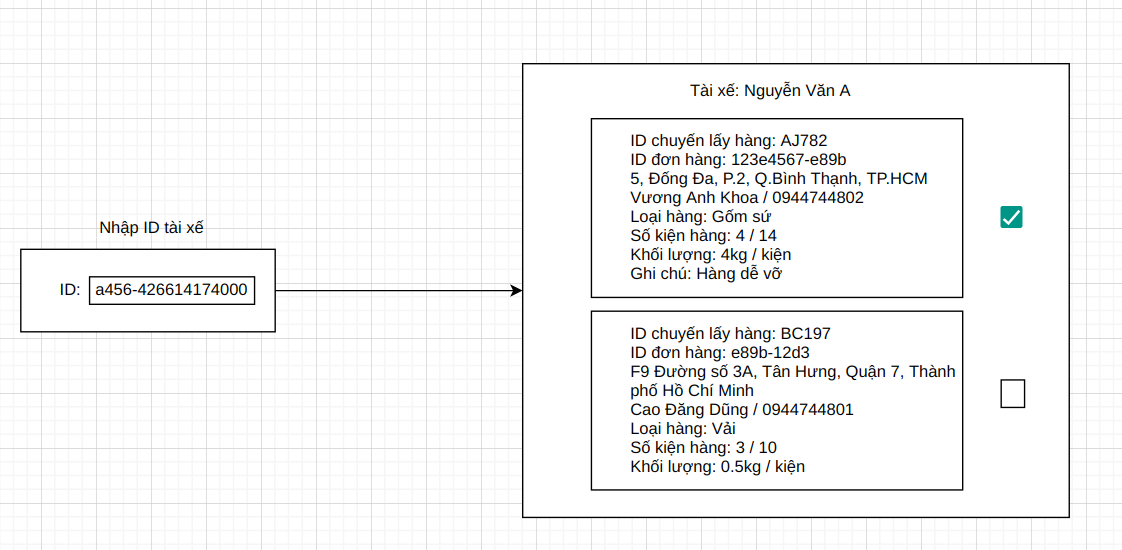
\includegraphics[width=1\textwidth]{/xacnhankienhangvaokho.png}
			\centering
			\linebreak
			\caption{Wireframe xác nhận kiện hàng vào kho}
		\end{figure}
		
		\item \textbf{Xác nhận đơn hàng xuất kho}: Khi tài xế liên tỉnh xuất kho đến yêu cầu thủ kho những đơn hàng cần giao liên tỉnh thì thủ kho sẽ search ID của tài xế liên tỉnh đó và xem được list các đơn hàng mà tài xế liên tỉnh đó được phân phối. Khi tài xế liên tỉnh chuyển những đơn hàng đó lên xe liên tỉnh thì thủ kho sẽ check vào những kiện hàng sẽ lên xe để hoàn tất quá trình xuất kho của kiện hàng. Việc check như vậy sẽ cập nhật trạng thái của đơn hàng trên hệ thống (Đã vào kho tập trung 1 -> Đang giao liên tỉnh).
		\item \textbf{Xác nhận đơn hàng vào kho}: Khi tài xế liên tỉnh đến kho, thủ kho sẽ search ID của tài xế liên tỉnh để xem list đơn hàng được phân công của tài xế Thủ kho sẽ kiểm tra xe của tài xế và check vào những đơn hàng thật sự có trong xe để hoàn tất quá trình nhập kho của đơn hàng.Trạng thái đơn hàng cập nhật từ (Đang giao liên tỉnh -> Đã vào kho tập trung 2). Nếu người gửi chọn option tự gửi đến kho, thủ kho sẽ search ID của người gửi và thực hiện tiếp các bước như trên. 
		
		\newpage
		
		\begin{figure}[!ht]
			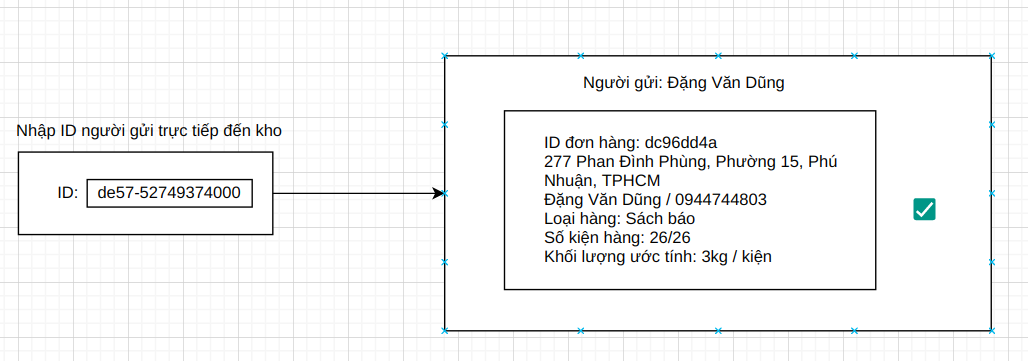
\includegraphics[width=1\textwidth]{/xacnhandonhangvaokho.png}
			\centering
			\linebreak
			\caption{Wireframe xác nhận đơn hàng vào kho}
		\end{figure}
		
		\item \textbf{Xác nhận kiện hàng xuất kho}: Khi tài xế nội tỉnh đến yêu cầu thủ kho những kiện hàng cần giao nội tỉnh thì thủ kho sẽ search ID của tài xế nội tỉnh đó và xem được list các kiện hàng mà tài xế nội tỉnh đó được phân phối. Khi tài xế nội tỉnh chuyển những kiện hàng đó lên xe nội tỉnh thì thủ kho sẽ check những kiện hàng trong list xem ở trên để xác nhận việc tài xế nội tỉnh đã chất hàng lên xe. Việc check như vậy sẽ cập nhật trạng thái của đơn hàng trên hệ thống (Đã vào kho tập trung 2 -> Đang giao hàng (x/tổng số kiện)).
	\end{itemize}
% 	\subsection{Hệ thống thông báo}
	\textbf{Gửi thông báo đến mail người dùng cho mỗi mức chuyển trạng thái}: Hệ thống sẽ gửi mail đến người dùng mỗi khi đơn hàng chuyển qua một trạng thái
	
	\begin{figure}[!ht]
		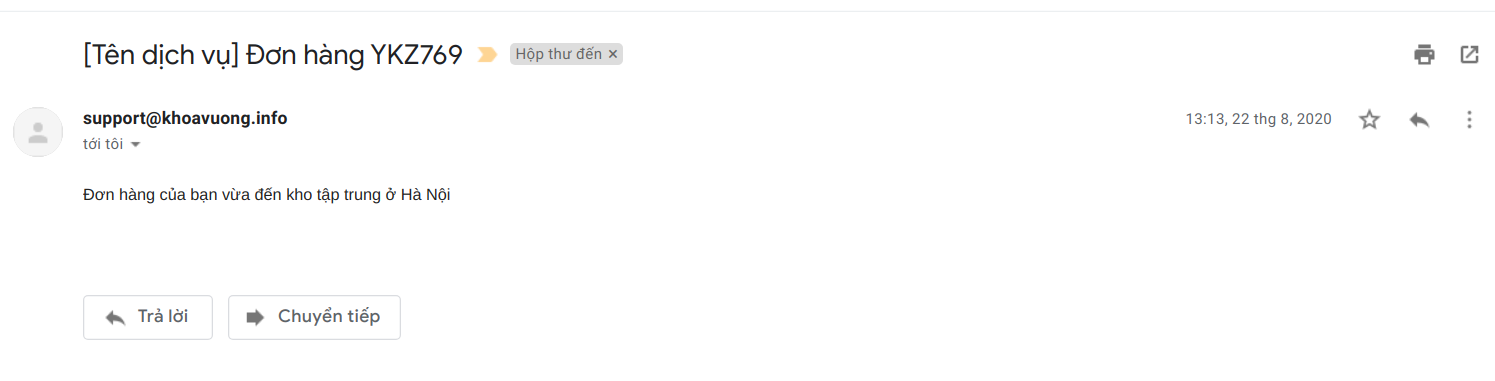
\includegraphics[width=1\textwidth]{/mail.png}
		\centering
		\linebreak
		\caption{Ví dụ mail thông báo dự kiến khi đơn hàng chuyển trạng thái}
	\end{figure}
	
\end{itemize}



% \subsection{Lược đồ ERD}
    \begin{figure}[!ht]
		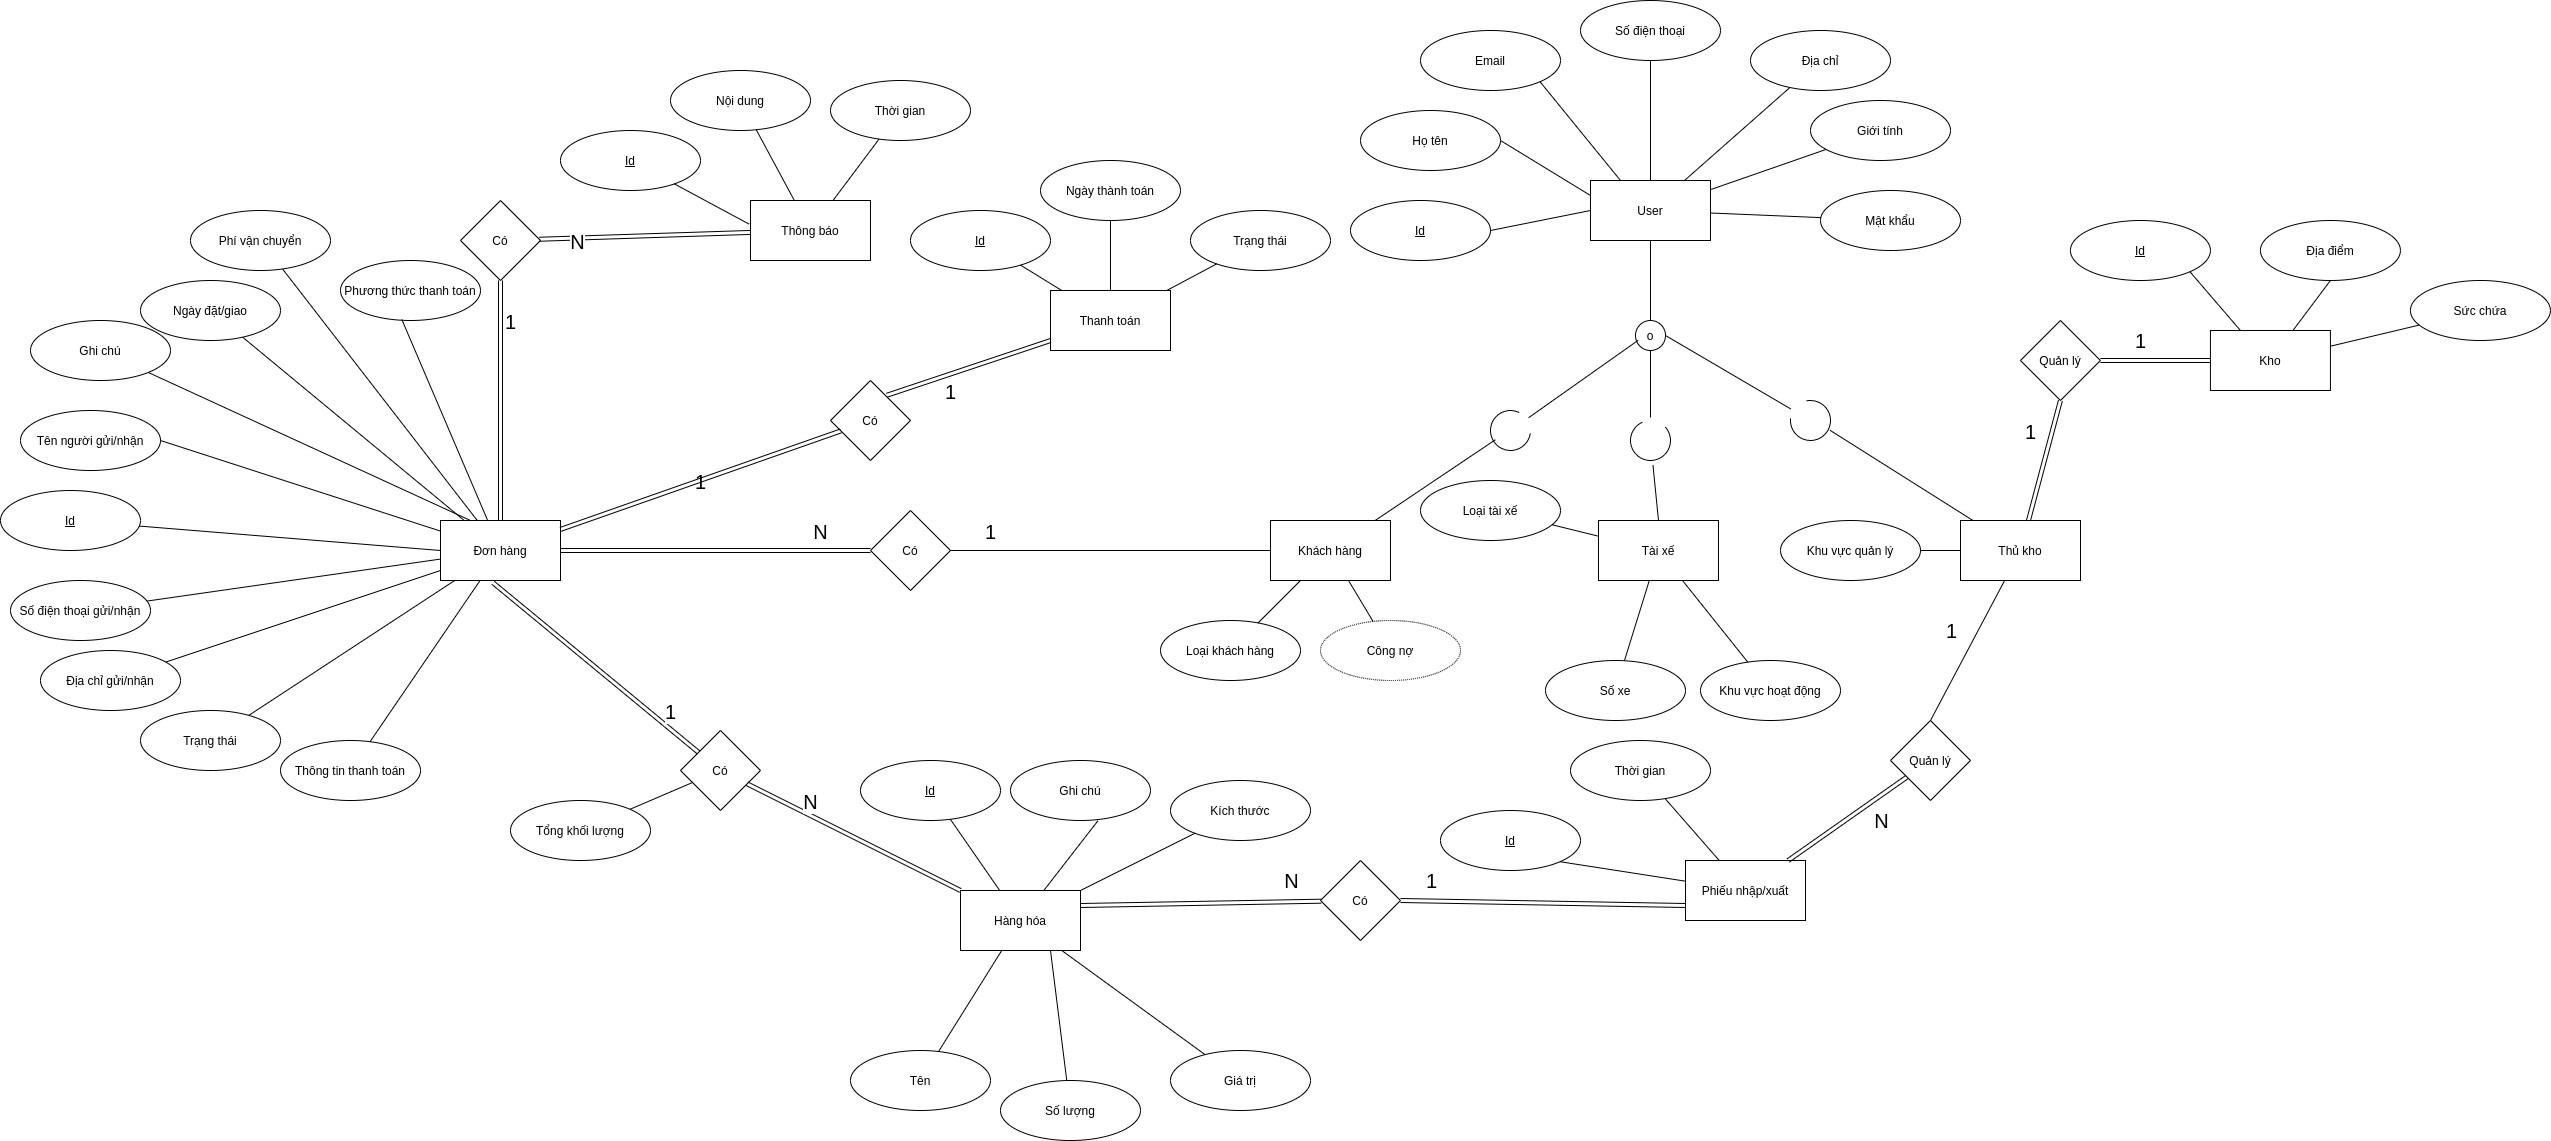
\includegraphics[width=1\textwidth]{Images/erd.jpg}
		\centering
		\linebreak
		\caption{Lược đồ ERD}
	\end{figure}
	
	
	
	
	\subsection{Thiết kế cơ sở dữ liệu}



	